% Für Bindekorrektur als optionales Argument "BCORfaktormitmaßeinheit", dann
% sieht auch Option "twoside" vernünftig aus
% Näheres zu "scrartcl" bzw. "scrreprt" und "scrbook" siehe KOMA-Skript Doku
\documentclass[12pt,a4paper,titlepage,headinclude,bibtotoc]{scrartcl}


%---- Allgemeine Layout Einstellungen ------------------------------------------

% Für Kopf und Fußzeilen, siehe auch KOMA-Skript Doku
\usepackage[komastyle]{scrpage2}
\pagestyle{scrheadings}
\automark[section]{chapter}
\setheadsepline{0.5pt}[\color{black}]

%keine Einrückung
\parindent0pt

%Einstellungen für Figuren- und Tabellenbeschriftungen
\setkomafont{captionlabel}{\sffamily\bfseries}
\setcapindent{0em}

\usepackage{caption}

%---- Weitere Pakete -----------------------------------------------------------
% Die Pakete sind alle in der TeX Live Distribution enthalten. Wichtige Adressen
% www.ctan.org, www.dante.de

% Sprachunterstützung
\usepackage[ngerman]{babel}

% Benutzung von Umlauten direkt im Text
% entweder "latin1" oder "utf8"
\usepackage[utf8]{inputenc}

% Pakete mit Mathesymbolen und zur Beseitigung von Schwächen der Mathe-Umgebung
\usepackage{latexsym,exscale,amssymb,amsmath}

% Weitere Symbole
\usepackage[nointegrals]{wasysym}
\usepackage{eurosym}

% Anderes Literaturverzeichnisformat
%\usepackage[square,sort&compress]{natbib}

% Für Farbe
\usepackage{color}

% Zur Graphikausgabe
%Beipiel: \includegraphics[width=\textwidth]{grafik.png}
\usepackage{graphicx}

% Text umfließt Graphiken und Tabellen
% Beispiel:
% \begin{wrapfigure}[Zeilenanzahl]{"l" oder "r"}{breite}
%   \centering
%   \includegraphics[width=...]{grafik}
%   \caption{Beschriftung} 
%   \label{fig:grafik}
% \end{wrapfigure}
\usepackage{wrapfig}

% Mehrere Abbildungen nebeneinander
% Beispiel:
% \begin{figure}[htb]
%   \centering
%   \subfigure[Beschriftung 1\label{fig:label1}]
%   {\includegraphics[width=0.49\textwidth]{grafik1}}
%   \hfill
%   \subfigure[Beschriftung 2\label{fig:label2}]
%   {\includegraphics[width=0.49\textwidth]{grafik2}}
%   \caption{Beschriftung allgemein}
%   \label{fig:label-gesamt}
% \end{figure}
\usepackage{subfigure}
\usepackage{adjustbox}

% Caption neben Abbildung
% Beispiel:
% \sidecaptionvpos{figure}{"c" oder "t" oder "b"}
% \begin{SCfigure}[rel. Breite (normalerweise = 1)][hbt]
%   \centering
%   \includegraphics[width=0.5\textwidth]{grafik.png}
%   \caption{Beschreibung}
%   \label{fig:}
% \end{SCfigure}
\usepackage{sidecap}

\usepackage{rotating}

% Befehl für "Entspricht"-Zeiche\resizebox{angle=90}n
\newcommand{\corresponds}{\ensuremath{\mathrel{\widehat{=}}}}

%Für chemische Formeln (von www.dante.de)
%% Anpassung an LaTeX(2e) von Bernd Raichle
\makeatletter
\DeclareRobustCommand{\chemical}[1]{%
  {\(\m@th
   \edef\resetfontdimens{\noexpand\)%
       \fontdimen16\textfont2=\the\fontdimen16\textfont2
       \fontdimen17\textfont2=\the\fontdimen17\textfont2\relax}%
   \fontdimen16\textfont2=2.7pt \fontdimen17\textfont2=2.7pt
   \mathrm{#1}%
   \resetfontdimens}}
\makeatother

%Si Einheiten
\usepackage{siunitx}

%c++ Code einbinden
\usepackage{listings}
\lstset{numbers=left, numberstyle=\tiny, numbersep=5pt}

%Differential
\newcommand{\dif}{\ensuremath{\mathrm{d}}}

%Boxen,etc.
\usepackage{fancybox}
\usepackage{empheq}

%Fußnoten auf gleiche Seite
\interfootnotelinepenalty=1000

%Dateien aus Unterverzeichnissen
\usepackage{import}

%Bibliography \bibliography{literatur} und \cite{gerthsen}
%\usepackage{cite}
\usepackage{babelbib}
\selectbiblanguage{ngerman}

\begin{document}

\begin{titlepage}
\centering
\textsc{\Large Anfängerpraktikum der Fakultät für
  Physik,\\[1.5ex] Universität Göttingen}

\vspace*{4.2cm}

\rule{\textwidth}{1pt}\\[0.5cm]
{\huge \bfseries
  Das Prismen- und\\[1.5ex]
  Gitterspektrometer}\\[0.5cm]
\rule{\textwidth}{1pt}

\vspace*{3.0cm}

\begin{Large}
\begin{tabular}{ll}
Praktikant:
 	&  Felix Kurtz\\
 	&  Michael Lohmann\\

E-Mail: 
	&  felix.kurtz@stud.uni-goettingen.de\\
	& m.lohmann@stud.uni-goettingen.de\\

 Betreuer: & Phillip Bastian\\
 Versuchsdatum: &  05.03.2015\\
\end{tabular}
\end{Large}

\vspace*{0.8cm}

\begin{Large}
\fbox{
  \begin{minipage}[t][2.5cm][t]{6cm} 
    Testat:
  \end{minipage}
}
\end{Large}

\end{titlepage}

\tableofcontents

\newpage

\section{Einleitung}
\label{sec:einleitung}
Mit einem Gitter kann man durch Interferenzeffekte weißes Licht in seine Spektralfarben zerlegt werden.
Das Gleiche kann man auch auf Grund der Dispersion mit einem Prisma tun.
In diesem Versuch sollen an einer Quecksilber-Dampflampe beide Verfahren  bezüglich des Auflösungsvermögens verglichen werden.

\section{Theorie}
\label{sec:theorie}
\subsection{Prismenspektrometer}

\begin{figure}[!h]
	\centering
	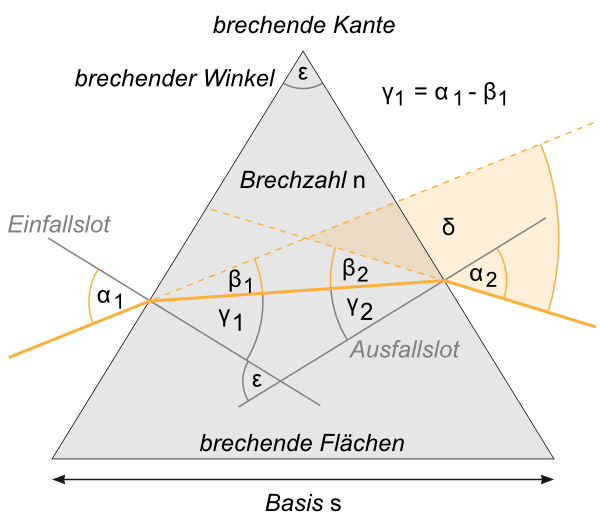
\includegraphics[scale=0.6]{Prisma.png}
	\caption{Prismaquerschnitt mit Strahlengang. \cite[Datum: 28.12.2014]{LP19}}
	\label{fig:prisma}
\end{figure}
Dieses Spektrometer basiert auf der \textit{Dispersion}, also der Wellenlängenabhängigkeit des Brechungsindex.
Unter \textit{normaler} Dispersion versteht man, dass der Brechungsindex $n$ mit zunehmender Wellenlänge abnimmt.
Bei anomaler Dispersion geschieht das Gegenteil: $\frac{\dif n}{\dif \lambda} > 0$.\\

Das \emph{Snellius'sches Brechungsgesetz} beschreibt, wie ein Strahl, der im Winkel $\alpha_1$ zum Lot auf eine Grenzschicht zwischen einem Medium mit Brechungsindex $n_1$ und einem mit einem Index $n_2$ trifft, gebrochen wird \cite[S.101]{hecht}:
\begin{align}
	n_1 \cdot \sin \alpha_1 = n_2 \cdot \sin \alpha_2 \,.
	\label{eq:Snellius} 
\end{align}
Im zweiten Medium verläuft der Strahl dann in einem Winkel $\alpha_2$ zum Lot.\\

Mit dem Brechungsgesetz  und den geometrischen Beziehungen aus Abb.\ref{fig:prisma} $\gamma_1+\gamma_2=\varepsilon$ sowie $\delta=\alpha_1+\alpha_2-\epsilon$ folgt bei symmetrischer Durchstrahlung ($\alpha_1=\alpha_2$) für den Ablenkwinkel $\delta$ (vgl. \cite[S.187f.]{hecht})

\begin{align}
	\sin\left(\frac{\delta+\varepsilon}{2}\right)=n\cdot\sin\left(\frac{\varepsilon}{2}\right)\,.
\end{align}

Dies leitet man nach $n$ ab und stellt nach $\frac{\dif \delta}{\dif n}$ um:
\begin{align}
	\frac{\dif \delta}{\dif n}=\frac{\sin\left(\frac{\varepsilon}{2}\right)}{\cos\left(\frac{\delta+\varepsilon}{2}\right)}=\frac{B}{S}
\end{align}

Damit kann man nun die Winkeldispersion berechnen:
\begin{align}
	D=\frac{\dif \delta}{\dif \lambda}=\frac{B}{S}\cdot\frac{\dif n}{\dif \lambda}\,.
	\label{eq:winkeldispersion}
\end{align}

\begin{figure}[!h]
	\centering
	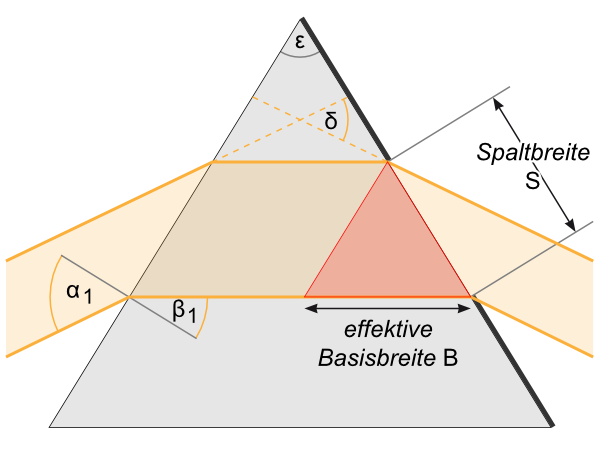
\includegraphics[scale=0.6]{Prisma2.png}
	\caption{Skizze zur Bestimmung des Auflösungsvermögens. \cite[Datum: 28.12.2014]{LP19}}
	\label{fig:prisma2}
\end{figure}

Das \textbf{Auflösungsvermögen} $A:=\frac{\lambda}{\Delta\lambda}$ charakterisiert, ob ein Spektrometer zwei unterschiedliche Wellenlängen auflösen kann.
Für das Prisma gilt dann:
\begin{align}
	A=B\left|\frac{\dif n}{\dif \lambda}\right|\,.
	\label{eq:aufloesungP}
\end{align}

\subsection{Gitterspektrometer}
Für ein Maximum muss der Wegunterschied ein ganzzahliges Vielfaches der Wellenlänge $\lambda$ sein, also $\Delta s=a \cdot \sin \alpha=k \lambda$.
Für Minima und Maxima gilt dann nach \cite[S.461ff.]{hecht}
\begin{align}
	\sin\alpha_\text{max}&=\frac{k\lambda}{a}\,,\\
	\sin\alpha_\text{min}&=\frac{n\lambda}{Na}\,.
\end{align}

Um zwei verschiedene Wellenlängen aufzulösen, muss das Maximum der einen Wellenlänge und das Minimum der anderen an gleicher Stelle liegen.
Somit ist das Auflösungsvermögen durch
\begin{align}
	A=kN
\end{align}
gegeben.
Dabei ist $k$ die Beugungsordnung und $N$ die Anzahl der beleuchteten Spalte.

\subsection{Quecksilber-Dampflampe}
Eine Quecksilber-Dampflampe hat kein kontinuierliches Spektrum wie etwa eine Glühbirne, sondern diskrete Linien.
In Tabelle \ref{tab:Hg-Linien} sind die für diesen Versuch wichtigen Linien aufgeführt.

\begin{table}
	\centering
	\begin{tabular}{|c|c|}
	    \hline		
		Farbe & Wellenlänge [nm]\\
		\hline
		\hline
		gelb & 579.07, 576.96\\
		\hline		
		grün & 546.07\\
		\hline
		violett & 407.78, 404.66\\
		\hline	
	\end{tabular}
	\caption{Für den Versuch wichtige Linien des Quecksilber-Spektrums}
	\label{tab:Hg-Linien}
\end{table}

\section{Durchführung}
\label{sec:durchfuehrung}

\begin{figure}[!h]
	\centering
	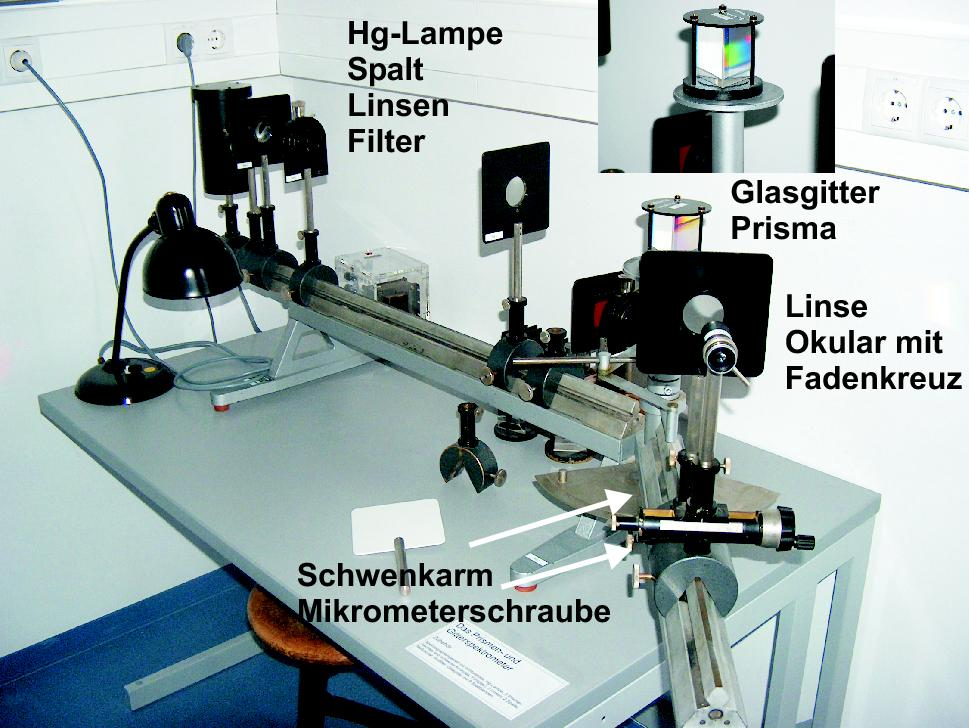
\includegraphics[scale=0.4]{Aufbau.jpg}
	\caption{Der Versuchsaufbau. \cite[Datum: 28.12.2014]{LP19}}
	\label{fig:aufbau}
\end{figure}

\subsection{Prismenspektrometer}
Folgende Schritte werden zuerst mit dem Kronglas-Prisma durchgeführt, danach mit dem Prisma aus schwerem Flintglas.
Bei beiden misst man die geometrischen Basislängen.\\

Zuerst wird der Spektralapparat aufgebaut und justiert.
Dazu werden die Hg-Lampe, die Kondensorlinse, der Beleuchtungsspalt sowie die zweite Linse in der gleichen Reihenfolge wie in Abb. \ref{fig:aufbau} befestigt - und zwar so, dass die Lichtstrahlen danach parallel sind.
Mit der dritten Linse und dem Okular wird der Spalt scharf abgebildet.
Zur späteren Auswertung werden die Brennweiten und Linsenpositionen notiert.
Nun wird das Fadenkreuz des Okulars auf den Strahl eingestellt und die Position der Winkelskala sowie des Feintriebs notiert.

Danach wird das Prisma in den Strahlengang gestellt und so gedreht, dass das Prisma symmetrisch durchstrahlt wird (minimaler Ablenkwinkel).
Der Schwenkarm wird nun auf eine der gelben Linien justiert.
Den Winkel notiert man.

Über den Abstand der eingestellten gelben Linie zur grünen Linie (Feintrieb des Okulars, der Schwenkarm wird nicht verstellt) und den Abstand der dritten Linse zum Okular kann der Ablenkwinkel $\Delta\varphi$ zwischen den beiden Linien bestimmt werden.

Nun verengt man den Strahl mit einem zweiten Spalt vor dem Prisma gerade so, dass die beiden gelben Linien noch getrennt erscheinen.
Dieser Spalt ersetzt nun den Eingangsspalt, das Prisma wird entfernt und durch den Rotfilter ersetzt, der Schwenkarm wird zurückgeschwenkt.
Mit dem Messokular vermisst man nun das Spaltbild.

\subsection{Gitterspektrometer}
Nun benutzt man das Glasgitter, welches sehr empfindlich ist und nicht berührt werden darf.

Der Aufbau ist der gleiche wie im obigen Abschnitt.
Es wird lediglich das Gitter anstelle des Prismas gesetzt -- möglichst senkrecht zum Strahl.
Für die erste, vierte und achte Ordnung werden die Ablenkwinkel der grünen Linie sowie der gelben und violetten Doppellinien bestimmt.

Für die 1., 4. und 8. Ordnung der beiden gelben Linien wird in die Plexiglasführung nacheinander kleinere Spaltblenden eingeführt und so die Blende $d_\text{min}$ bestimmt, so dass die beiden Linien gerade nicht mehr getrennt aufgelöst werden.

\section{Auswertung}
\label{sec:auswertung}

\subsection{Prismenspektrometer}
\subsubsection{Strahlengänge}
Die Abbildungen \ref{fig:Strahlengang1} und \ref{fig:Strahlengang2} zeigen, wie der Aufbau montiert war.
Zuerst wird das Licht der Hg-Lampe mit der Kondensorlinse auf einen Spalt abgebildet.
Die zweite Linse hat einen Abstand $f_2$ von diesem.
\begin{figure}[!htb]
	\def\svgwidth{0.8\linewidth}	
	\input{strahlengang1.pdf_tex}
	\caption{Strahlengang zur Justage. \protect \footnotemark}
	\label{fig:Strahlengang1}	
\end{figure}
\footnotetext{von http://genug-davon.de/aprakt/index.php?section=v19}

\begin{figure}[!htb]
	\def\svgwidth{0.8\linewidth}
	\input{strahlengang2.pdf_tex}
	\caption{Strahlengang des Prismenspektrometers.  \protect \footnotemark[1]}
	\label{fig:Strahlengang2}
\end{figure}

\subsubsection{Winkeldispersion}
Die Winkeldispersion wird als konstant angenommen.
Also kann man sie berechnen, indem man den Winkelunterschied $\Delta\delta$ durch den Wellenlängenunterschied $\Delta\lambda$ teilt.
Mit der Kleinwinkelnäherung ist $\Delta\delta=\frac{\Delta x}{s}$ und der Fehlerfortpflanzung folgen
\begin{align}
	D&=\frac{x_\text{gelb} - x_\text{grün}}{\Delta\lambda \cdot s}\,\text{und}\\
\sigma_{D}&=\frac{1}{\Delta\lambda \cdot s^{2}} \cdot \sqrt{2s^{2} \cdot \sigma_{x} + \sigma_{s}^{2} \cdot \left(x_\text{gelb} - x_\text{grün}\right)^{2}}\,.
\end{align}
Dabei ist $s$ der Abstand zwischen dritter Linse und Okular, $\Delta x$ ist der Wegunterschied der am Feintrieb abgelesen wurde.
\begin{table}[!htb]
	\centering
	\begin{tabular}{|c|c|c|}
		\hline
		Glas & \multicolumn{2}{c|}{Winkeldispersion}\\		
		 & Literaturwert [$10^6~^\circ$/m] & Messwert [$10^6~^\circ$/m]\\
		\hline
		Kronglas& 3.47 & $4.33 \pm 0.19$ \\
		Leichtes Flintglas & 9.01 & $8.45 \pm 0.22$ \\
		Schweres Flintglas & 15.0 & $13.39 \pm 0.26$ \\
		\hline
	\end{tabular}
	\caption{Winkeldispersion der drei Prismenmaterialien}
	\label{tab:Dispersion}
\end{table}

\subsubsection{Auflösungsvermögen}
Die zweite Linse hat laut Angabe eine Brennweite von $f_2=(29.8 \pm 0.3)~$cm.
Für das Prisma aus leichtem Flintglas wurde als Bild des Spaltes, bei dem die zwei gelben Linien gerade nicht mehr aufgelöst werden, eine Breite von $B'=(0.55 \pm 0.03)~$mm gemessen.
Die tatsächliche Strahlbreite $S$ ergibt sich als Bildgröße durch Vergrößerung des optischen Systems.
Dabei wird die Vergrößerung als Quotient des Abstandes der dritten Linse zum Okular (Bildweite $b=(30.5\pm 0.5)~$mm) durch die Brennweite der zweiten Linse, hier der Gegenstandsweite, berechnet.
Mit der Fehlerfortpflanzung ergeben sich also folgende Formeln:
\begin{align}
	S&=B'\cdot\frac{f_2}{b}\\
	\sigma_S&=\sqrt{\left(\frac{f_2}{b}\right)^2\sigma_{B'}^2+\left(\frac{B'}{b}\right)^2\sigma_{f_2}^2+\left(\frac{B' \cdot f_2}{b^2}\right)^2\sigma_b^2}\,.
\end{align}
Dann erhält man $S=(0.55\pm 0.11)~$mm.\\
Bei dem Prisma aus Kronglas konnte man den Spalt nicht so weit aufdrehen, dass man zwei Linien gesehen hat.
Mit den beiliegenden Blenden haben wir festgestellt, dass die Spaltbreite größer als 2.75 mm sein müsste.

\begin{align}
\sigma_{A}=\sqrt{D^{2} \cdot \sigma_{S}^{2} + S^{2} \cdot \sigma_{D}^{2}}
\end{align}

\begin{table}[!htb]
	\centering
	\begin{tabular}{|c|c|c|c|}
		\hline		
		& theoretischer Wert & leichtes Flintglas &  Kronglas \\
		\hline
	    Auflösungsvermögen & $274.44$ & $81 \pm 17$ & $>208$ \\
		\hline		
	\end{tabular}
	\caption{Prismenspektrometer: Auflösungsvermögen}
	\label{tab:prismaA}
\end{table}

\subsubsection{Grenzen der Auflösung}

\begin{align}
	S&=B \cdot \cos{\left (\frac{\delta+\epsilon}{2}\right )}\\
\sigma_{S}&=\frac{1}{2} \cdot \sqrt{B^{2} \cdot \sigma_{\delta}^{2} \cdot \sin^{2}{\left (\frac{\delta+\epsilon}{2} \right )} + 4 \cdot \sigma_{B}^{2} \cdot \cos^{2}{\left (\frac{\delta+\epsilon}{2} \right )}}
\end{align}

\begin{table}[!htb]
	\centering
	\begin{tabular}{|c|c|c|c|}
		\hline		
		& Kronglas & leichtes Flintglas & schweres Flintglas \\
		\hline
	    Ablenkwinkel $\delta$ & $(38.7\pm 0.1)^\circ$ &  $(51.9\pm 0.1)^\circ$ & $(65.0\pm 0.1)^\circ$ \\
	    Basisbreite $B$ & $(5.2 \pm 0.1)~$cm & $(5.2 \pm 0.2)~$cm &$(6.0 \pm 0.2)~$cm \\
	    maximale Spaltbreite $S$ & $(3.39 \pm 0.07)~$cm & $(2.86 \pm 0.09)~$cm & $(2.91 \pm 0.11)~$cm \\
	    Auflösungsvermögen A& $2560 \pm 120$ & $4220 \pm 180$ & $6800 \pm 290$ \\
		kleinstes $\Delta \lambda$ bei $\lambda=579.07~$nm& $(230 \pm 10)~$pm & $(137 \pm 6)~$pm& $(85 \pm 4)~$pm \\
		\hline
	\end{tabular}
\end{table}

\subsection{Gitterspektrometer}
\subsubsection{Gitterkonstante}
\begin{align}
	a&=\frac{k \cdot \lambda}{\sin{\left (\alpha \right )}}\\
	\sigma_{a}&=\frac{k \cdot \lambda \cdot \sigma_{\alpha}}{\sin^{2}{\left (\alpha \right )}} \cdot \left\lvert{\cos{\left (\alpha \right )}}\right\rvert
\end{align}


\begin{table}[!htb]
	\centering	
	\begin{tabular}{|c|c|c|c|c|c|c|}
		\hline
		&Farbe & violett & violett & grün & gelb & gelb \\
		& $\lambda$ [nm]& 404.66 & 407.78 & 546.07 & 576.96 & 579.07\\
		\hline
		1.Ordnung & $\alpha$ $[^\circ]$ & $2.40 \pm 0.10$ & $2.40 \pm 0.10$ & $3.20 \pm 0.10$ & $3.40 \pm 0.10$ & $3.40 \pm 0.10$ \\ 
		& $a$ [$\mu$m] & $10.1 \pm 0.4$ & $10.2 \pm 0.4$ & $10.1 \pm 0.4$ & $10.0 \pm 0.3$ & $10.1 \pm 0.3$\\
		\hline
		4.Ordnung & $\alpha$ $[^\circ]$  & $9.30 \pm 0.10$
& $10.00 \pm 0.10$ & $12.60 \pm 0.10$ & $13.30 \pm 0.10$ & $13.40 \pm 0.10$ \\
		& $a$ [$\mu$m] & $10.02 \pm 0.11$ & $9.39 \pm 0.09$ & $10.01 \pm 0.08$ & $10.03 \pm 0.07$ & $9.99 \pm 0.07$ \\
		\hline
		8.Ordnung & $\alpha$ $[^\circ]$ & $20.50 \pm 0.10$
& $20.50 \pm 0.10$ & $26.10 \pm 0.10$ & $27.70 \pm 0.10$ & $27.90 \pm 0.10$ \\
		& $a$ [$\mu$m] & $9.24 \pm 0.04$ & $9.32 \pm 0.04$ & $9.93 \pm 0.04$ & $9.93 \pm 0.04$ & $9.90 \pm 0.04$ \\
		\hline
	\end{tabular}
	\caption{Gitter: Beugungswinkel und daraus berechnete Gitterkonstante}
	\label{tab:gitter}
\end{table}

Als gewichteter Mittelwert aus allen Messungen ergibt sich für die Gitterkonstante ein Wert von $a=(9.769 \pm 0.015)~\si{\micro\meter}$.
Da die Messung der violetten Linien teilweise sehr abweichende Werte liefert, wird für alle weiteren Rechnungen der gewichtete Mittelwert aus Messungen der gelben sowie grünen Linien für die Gitterkonstante genommen: 
\begin{empheq}[box=\shadowbox]{align*}
	a=(9.936 \pm 0.018)~\si{\micro\meter}\,.
\end{empheq}

\subsubsection{Wellenlängenunterschied der gelben Linien}
\begin{align}
	\frac{k\lambda}{a}&=\sin\alpha \\
	\frac{k(\lambda+\Delta\lambda)}{a}&=\sin(\alpha+\Delta\alpha) =\sin\alpha\cdot\cos\Delta\alpha +\cos\alpha\cdot\sin\Delta\alpha \approx\sin\alpha+ \cos\alpha\cdot\Delta\alpha
\end{align}

\begin{align}
	\Delta\lambda&=\frac{a}{k} \cdot \Delta \alpha \cdot \cos{\left (\alpha \right )}\\
\sigma_{\Delta\lambda}&=\frac{a}{k} \cdot \sigma_{\Delta \alpha} \cdot \left\lvert{\cos{\left (\alpha \right )}}\right\rvert
\end{align}

Für die 4.Beugungsordnung ergibt sich eine Differenz von $\Delta\lambda=(4.2 \pm 4.2)~$nm, für die 8. Beugungsordnung eine von $\Delta\lambda=(3.8 \pm 1.9)~$nm.
Der tatsächliche Wert liegt bei  $\Delta\lambda=2.11~$nm.

\subsubsection{Wellenlänge der violetten Doppellinie}
\begin{align}
	\lambda_\text{violett}&=\frac{a}{k} \cdot \sin{\left (\alpha \right )}\\
\sigma_{\lambda_\text{violett}}&=\frac{1}{k} \cdot \sqrt{a^{2} \cdot \sigma_{\alpha}^{2} \cdot \cos^{2}{\left (\alpha \right )} + \sigma_{a}^{2} \cdot \sin^{2}{\left (\alpha \right )}}
\end{align}

\begin{table}[!htb]
	\centering
	\begin{tabular}{|c|c|c|c|c|}
		\hline
		& 1.Ordnung & \multicolumn{2}{c|}{4.Ordnung} & 8.Ordnung\\
	    & & 1.Wert & 2.Wert & \\
		\hline
		$\lambda_\text{violett}$ & $(410 \pm 20)~$nm & $(404 \pm 5)~$nm & $(431 \pm 5)~$nm & $(435.0 \pm 2.2)~$nm  \\
		\hline
	\end{tabular}
	\caption{Wellenlänge der violetten Doppellinie}
	\label{tab:violett}
\end{table}

\subsubsection{Auflösungsvermögen}
\begin{table}[!htb]
	\centering
	\begin{tabular}{|c|c|c|c|c|}
		\hline
		& benötigter Wert &1.Ordnung &  4.Ordnung & 8.Ordnung \\
		\hline
	    Auflösungsvermögen & $274.44$ & $>257$ & $308.6 \pm 0.5$ & $<617$ \\
		\hline
	\end{tabular}
	\caption{Gitter: Auflösungsvermögen}
	\label{tab:gitterA}
\end{table}
Das maximales Auflösungsvermögen in der ersten Ordnung beträgt $A=1542.89 \pm 2.4$.
Dies wird dann erreicht, wenn das Gitter in seiner ganzen Breite von $1.5~$cm beleuchtet wird.

\section{Diskussion}
\label{sec:diskussion}
\subsection{Prismenspektrometer}
Der Wert der Winkeldispersion weicht für Kronglas etwa $25\%$, für leichtes Flintglas etwa $6\%$ und für schweres Flintglas  um circa $11\%$ vom jeweiligen Literaturwert ab.
Außerdem wurden die Fehler unterschätzt, da die tatsächlichen Werte nicht in den Fehlerintervallen liegen.
Eventuell ist die Winkeldispersion der Prismen nicht wie angenommen konstant, was diese Abweichungen zum Teil erklären würde.
Ein weiterer Grund könnte das nicht ganz parallele Licht gewesen sein.
So ist die Umrechnung der Feintriebdifferenz in eine Winkeldifferenz fehlerhaft.\\

Für das Auflösungsvermögen des Flintglas-Prismas wurde ein mehr als dreimal so kleiner Wert als der für die beiden gelben Linien benötigte gemessen.
Dies kann nicht sein, lässt sich aber damit erklären, dass für die mit dem Feintrieb bestimmte Breite des Spalts $B'$ nicht -- wie notiert -- $0.55~$mm gemessen wurde, sondern $1.55~$mm.
Dann verdreifacht sich das Auflösungsvermögen in etwa.
Bei dem Prisma aus Kronglas konnte nur abgeschätzt werden, da man auch bei ganz geöffneter Stellung des zweiten verstellbaren Spalts die zwei Linien nicht getrennt sehen konnte.
So haben wir die Blenden, die eigentlich für das Gitter bestimmt waren, genutzt.
Aber auch hier hat eine Breite von $2.75~$mm nicht genügt.
Später wurde uns bewusst, dass der Beleuchtungsspalt viel weiter auf geht und mit dem anderen getauscht hätte werden müssen.\\

Das maximale Auflösungsvermögen zu erreichen ist mit diesem Aufbau sehr illusorisch, da man dafür einen parallelen kohärenten Strahl benötigt, der einige Zentimeter breit ist.
Erst dann wird das gesamte Prisma beleuchtet.
Wenn man dies aber hinbekäme könnte man mit dem Prisma aus schwerem Flintglas Wellenlängendifferenzen von weniger als einem Zehntel Nanometer auflösen.

\subsection{Gitterspektrometer}
Bei einem Wert von $a=(9.936 \pm 0.018)~\si{\micro\meter}$ für die Gitterkonstante kann man davon ausgehen, dass der tatsächliche Wert $a=10~\si{\micro\meter}$ beträgt.
Dann weicht der errechnete Wert davon weniger als $1\%$ ab.
Jedoch wurden die Fehler unterschätzt, da der tatsächliche Wert nicht im Fehlerintervall liegt.
Ein Hauptgrund hierfür ist, dass der Offset ohne Fehler angenommen wurde.
Dieser kann aber das Ergebnis stark beeinflussen.
Außerdem ist auffällig, dass die aus den violetten Linien höherer Ordnung berechnete Gitterkonstante viel zu gering ist.
Dies lässt sich damit erklären, dass falsch gezählt wurde.\\

Der Wellenlängenunterschied der gelben Linien ist mit einem sehr großen Fehler behaftet, da die Winkeldifferenz in etwa genauso groß ist wie der Messfehler von $0.1^\circ$
Trotzdem liegt der bestimmte Wert in der Größenordnung des tatsächlichen Wertes.
Er weicht in etwa um $100\%$ ab, aber der tatsächliche Wert liegt im Fehlerintervall.
Man hätte die Differenz genauer bestimmen können, wenn man mit dem Feintrieb gearbeitet hätte.\\

Die Wellenlänge der violetten Doppellinie wurde aus der ersten und dem ersten Wert der vierten Beugungsordnung gut bestimmt: Beide Werte weisen eine Differenz von weniger als $2\%$ vom Literaturwert $\lambda_1=407.78~$nm, $ \lambda_2=404.66~$nm auf.
Außerdem liegen die tatsächlichen Werte im Fehlerintervall.
Die anderen beiden Messwerte sind mehr als $5\%$ zu groß.
Dies lässt sich wieder damit erklären, dass falsch gezählt wurde.
Vermutlich wurde die hellere blaue Linie $\lambda=435.84~$nm vermessen.\\

Das benötigte Auflösungsvermögen, um die zwei gelben Linien noch getrennt sehen zu können, wurde in der ersten Ordnung auch nicht mit der größten Blende erreicht, so konnte nur abgeschätzt werden.
In der 8. Ordnung hingegen konnte man mit der $0.75~$mm breiten Linie wie zuvor in der vierten Ordnung beide Linien getrennt sehen.
Setze man aber die etwas kleinere $0.5~$mm-Blende ein, wurde das Bild schwarz.
Der Spalt wurde also nicht beleuchtet.
So konnte wieder nur abgeschätzt werden.
Beide Abschätzungen stimmen mit der Theorie überein.

\bibliography{literatur}
\bibliographystyle{babalpha}

\end{document}
